\htwo{Open Secure Sockets Layer}
\sectionauthor{Mario Naunović}
\hthree{Allgemein}

OpenSSL ist eine freie Software unter der OpenSSL-Lizenz (seit Version 3.0 Apache Lizenz), die SSL und TLS implementiert. Zusätzlich sind weitere Implementierungen von verschiedenen Verschlüsselungen wie AES, Blowfish, Triple DES und viele mehr. Weiters bietet OpenSSL eine Bibliothek mit Hashfunktionen an. Primär wird OpenSSL genutzt, um Keys zum Verschlüsseln udn Entschlüsseln sowie TLS-Zertifikate zu erstellen. 

\hthree{Transport Layer Security}

\hfour{Allgemeines über TLS}

TLS ist ein Verschlüsselungsprotokoll, um Kommunikation über das Internet zu verschlüsseln und die Kommunikationspartner zu authentifizieren. Dabei wird das Protokoll meistens mit HTTPS zusammen verwendet. TLS ist ebenfalls bekannt unter dem früheren Namen SSL.  

\begin{figure}[H]
    \centering
    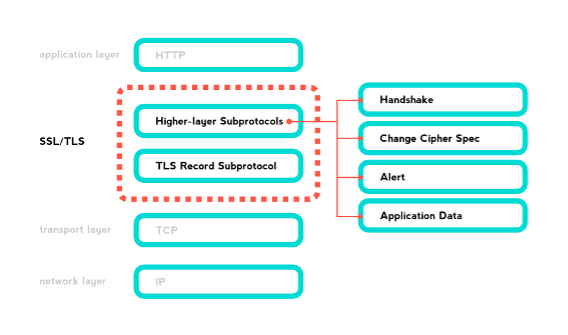
\includegraphics{media/OpenSSL/info.png}
    \caption{Lokation von TLS im ISO/OSI Schichtenmodell}
\end{figure}

TLS befindet sich im Bezug auf das ISO/OSI Schichtenmodell zwischen dem Transport Layer und dem Application Layer.

\hfour{Geschichte}

Im Jahr 1991 begann an der Universität von Texas die Entwicklung eines Netzwerkprotokolls, dass verschlüsselte Kommunikation unterstützt. Der Unterschied zu den bereits vorhandenen verschlüsselten Netzwerkprotokollen ist das Interface, dass die Verwendung durch die verschiedensten Internetapplikationen ermöglichen soll. Im Jahre 1994 stellte die Firma "Netscape Communications" die erste Version unter dem Namen SSL v1.0 fertig, diese wurde jedoch aufgrund von einer großen Anzahl an Schwachstellen nie veröffentlicht. Fünf Monate später wurde eine verbesserte Version unter dem Namen SSL v2.0 veröffentlicht. Im Jahre 1996 wurde SSL v3.0 veröffentlicht, und Netscape gab die Versionskontrolle an die Internet Engineering Task Force (IETF) ab, um einen Internet-Standard zu entwickeln. 1999 wurde TLS v1.0 veröffentlicht, welches eine verbesserte Version von SSL v3.0 ist. TLS v1.0 wurde etwas später durch viele RFCs erweitert, darunter Verschlüsselungen wie Triple-DES und AES. Seither wurden noch drei weitere Versionen veröffentlicht, die jeweils Schwachstellen beseitigt und zusätzliche Funktionalitäten bereitgestellt haben. Die letzte TLS Version ist Version 3.0, die am August 2018 veröffentlicht wurde. 

\hfour{Verbindungsaufbau und TLS-Handshake}
Damit über TLS kommuniziert werden kann, müssen die Kommunikationspartner zuerst zwei verschiedene Handshakes durchführen. 

\begin{figure}[H]
    \centering
    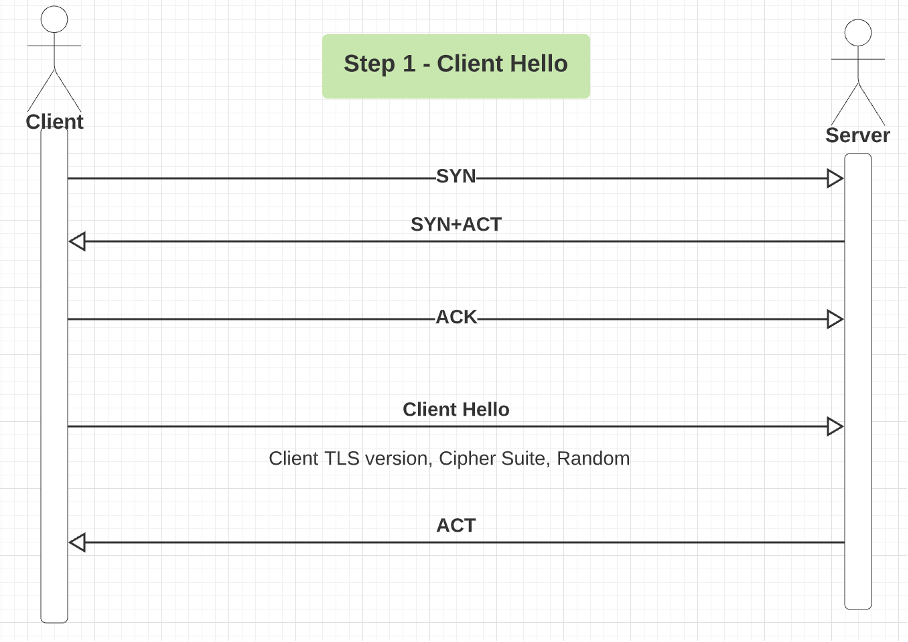
\includegraphics{media/OpenSSL/VerbindungsAufbau.png}
    \caption{Aufbau einer TLS Verbindung}
\end{figure}

Die Kommunikation beginnt damit, dass der Client den TCP-Handshake initiiert. Der Client schickt zuerst ein SYN-Paket. Falls der Server das SYN-Paket erhält, schickt er ein SYN-ACK-Paket zurück und lässt den Client somit wissen, dass sein SYN Paket angekommen ist. Damit dem Server bestätigt wird, dass sein SYN-ACK Paket angekommen ist, schickt der Client ein ACK-Paket. Nun ist der TCP-Handshake abgeschlossen und der Client kann mit dem TLS-Handshake beginnen. Als erstes schickt der Client ein "Client Hello"-Paket an den Server.

\begin{figure}[H]
    \centering
    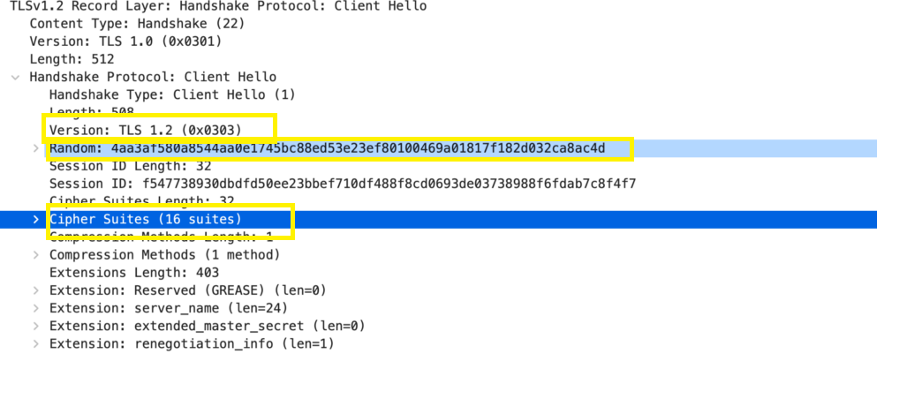
\includegraphics{media/OpenSSL/pt.png}
    \caption{Client-Hello Paket in PaketTracer}
\end{figure}

In diesem Paket sind Informationen wie die TLS-Version, ein zufällig generierter Wert und eine Liste von unterstützten "Cipher Suites". "Cipher Suites" legen fest, welche Algorithmen bei der sicheren Datenverbindung verwendet werden. Der zufällig generierte Wert, der beim "Client Hello"-Paket mitgeschickt wird, wird direkt beim Server selber gespeichert. Als Antwort schickt der Server ein "Server Hello"-Paket an den Client. 

\begin{figure}[H]
    \centering
    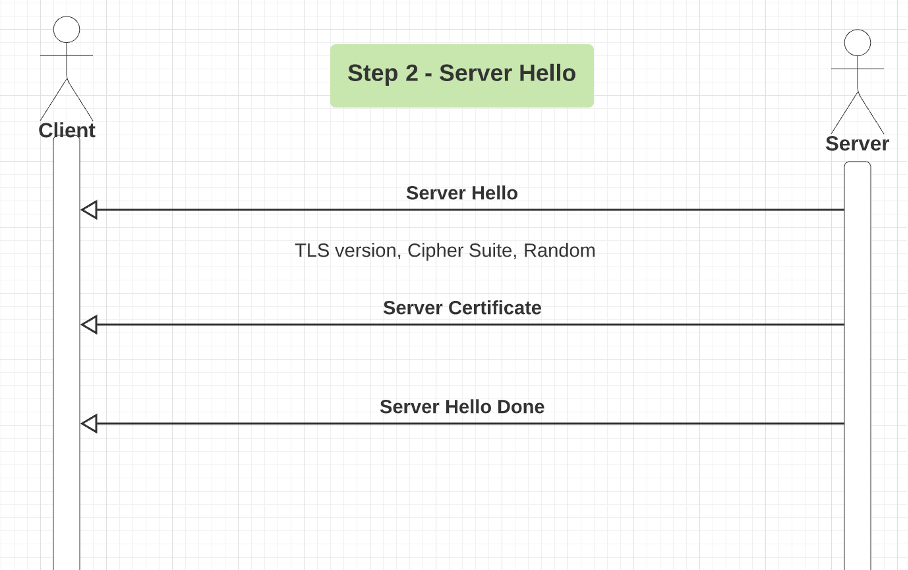
\includegraphics{media/OpenSSL/hello.png}
    \caption{Server-Hello Paket} 
\end{figure}

Der Server schickt die vom Client geschickte TLs-Version zurück, falls diese vom Server unterstüzt wird. Zusätzlich wird die vom Server bevorzugte "Cipher Suite" mitgeschickt, sowie ein zufälliger Wert, den der Client auf seinem Gerät speichert. Dann schickt der Server dem Client sein Zertifikat, um sich beim Client zu authentifizieren. Der Client muss dieses Zertifikat auf seine Richtigkeit überprüfen. Nachdem der Server dem Client sein Zertifikat schickt, sendet er zusätzlich noch eine "CertificateVerify"-Nachricht. Diese Nachricht enthält den gesamten vorherigen Nachrichtenaustausch zwischen Client und Server. Diesen Inhalt verschlüsselt der Server mit seinem Private-Key. Der Client kann nun die "CertificateVerify"- Nachricht mit dem Public-Key des Servers entschlüsseln und den darin enthaltenen Nachrichtenverlauf mit seinem Nachrichtenverlauf vergleichen. Damit kann der Client überprüfen, ob eine Nachricht von einer Drittperson verändert wurde und ob der Server wirklich im Besitz des Private-Keys ist. Optional kann der Server vom Client ein Zertifikat anfordern, damit sich der Client authentifiziert. 
Nachdem die "Hello"-Pakete und die Zertifikate ausgetauscht wurden, sind Client und Server bereit, die Parameter auszutauschen, die zur verschlüsselten Kommunikation erforderlich sind. Damit die endgültige Kommunikation nach dem Handshake verschlüsselt wird, werden symmetrische Verfahren wie zum Beispiel AES eingesetzt. Der Nachteil von symmetrischen Verfahren ist, dass beide Kommunikationspartner denselben Schlüssel zum Verschlüsseln bzw. Der Schlüssel muss also über Klartext übergeben werden. Um den Schlüssel beziehungsweise wichtige Parameter zur Berechnung des Schlüssels zu übergeben, wird dieser Schlüssel mithilfe eines Public-Key Verfahrens wie RSA oder Diffie-Hellman vor der Übertragung verschlüsselt. Der Grund, warum der eigentliche Datenaustausch nach dem TLS-Handshake nicht weiter mit einem asymmetrischen Verfahren verschlüsselt wird ist, dass asymmetrische Verschlüsselungen kompliziertere Rechenverfahren verwenden. Das Verschlüsseln und Entschlüsseln würden länger dauern als bei symmetrischen Verfahren.

\begin{itemize}
    \item Wird RSA verwendet, dann berechnet sich der Client einen zufälligen Wert, der "pre-master-secret" genannt wird. Diesen Wert verschlüsselt der Client dann mit dem Public-Key des Servers, den er durch das Zertifikat erhalten hat. In einer "Client Key Exchange Message" schickt der Client dann den verschlüsselten Wert an den Server. Der Server entschlüsselt die Nachricht nun mit seinem Private Key.
    \item Wird Diffie-Hellman verwendet, dann werden in der "Client Hello" und der "Server Hello" schon die benötigten Informationen für den Diffie-Hellman Schlüsselaustausch mitgegeben. Nun können Client und Server unabhängig voneinander das "pre-master-secret" berechnen.
\end{itemize}

Client und Server berechnen anschließend mithilfe von den zwei zufälligen Werten, die sie mithilfe der "Hello"-Nachrichten ausgetauscht haben und dem "pre-master-secret" das sogenannten "master-secret". Aus diesem "master-secret" können nun mehrere Schlüssel abgeleitet werden. Am Client werden der "client write key" und der "client write MAC key" erstellt. Am Server werden der "server write key" und der "server MAC key" erstellt. Der "server write key" und der "client write key" sind die symmetrischen Schlüssel, um den folgenden Datenverkehr zu verschlüsseln und zu entschlüsseln.

\begin{figure}[H]
    \centering
    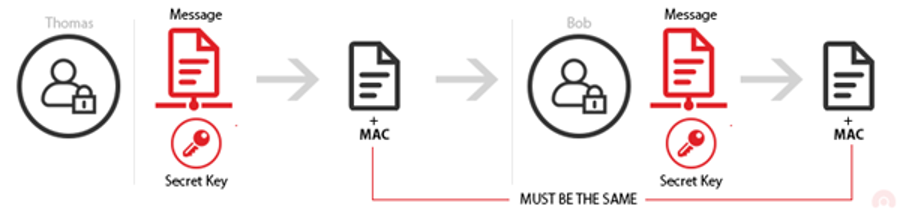
\includegraphics{media/OpenSSL/key.png}
    \caption{Prozess der Überprüfung} 
\end{figure}

Mithilfe der zwei "MAC"-Schlüssel können jeweils Client und Server Nachrichten auf ihre Authentizität prüfen. Wenn einer der Kommunikationspartner eine Nachricht senden will, verschlüsselt er deren Inhalt und fügt in ein MAC-Tag in das TLS-Paket ein. Der Empfänger berechnet sich ebenfalls mit seinem "MAC"-Schlüssel das MAC-Tag für die empfangenen Nachricht und vergleicht es mit dem "MAC"-Tag, dass der Absender berechnet hat. Wenn beide Tags übereinstimmen, ist die Authentizität der Nachricht gegeben.

Nachdem beide Kommunikationspartner die Schlüssel errechnet haben, schickt der Client eine "Change Cipher Spec"-Nachricht. Diese Nachricht teilt dem Server mit, dass der Client nun verschlüsselt kommuniziert. Nach der "Change Cipher Spec"-Nachricht schickt der Client eine "Finished"-Nachricht. Diese Nachricht ist bereits verschlüsselt und enthält das MAC-Tag. Der Server schickt nun auch eine "Change Cipher Spec" und eine "Finished" Nachricht. Nun ist der TLS-Handshake abgeschlossen und beide Kommunikationspartner können gesichert kommunizieren.

\hfour{Allgemeines über TLS-Zertifikate}

TLS-Zertifikate ermöglichen es Client und Server, sich zu identifizieren und zu beweisen. Zertifikate müssen außerdem von einer "Certificate Authority" signiert sein. 

\begin{figure}[H]
    \centering
    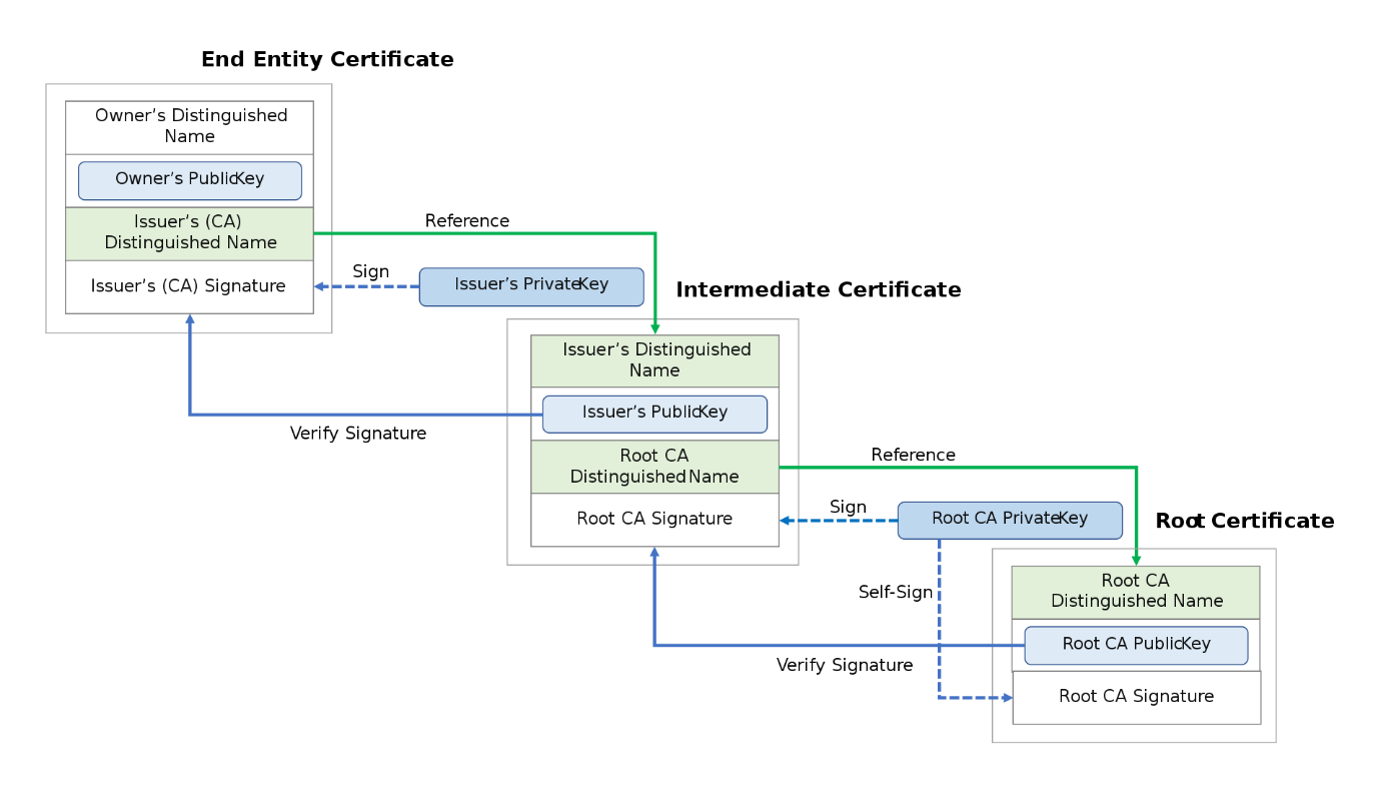
\includegraphics{media/OpenSSL/cert.png}
    \caption{TLS-Zertifikat Hierarchie}
\end{figure}

Ein wichtiges Element im Bezug auf Zertifikate ist die sogenannte "chain of trust". Sie ist ein hierarchisches Modell, dass das Vertrauen zwischen Zertifikaten darstellen soll. Das Zertifikat eines einfachen Clients oder Webserver wird "End Entity Certificate" genannt. Solche Zertifikate müssen von einer "Certificate Authority" ausgestellt werden. Die Zertifikate der "Certificate Authority" werden "Intermediate Certificate" genannt. Diese Zertifikate müssen wiederum von einer sogenannten "Root Certificate Authority" ausgestellt werden. Um ein Zertifikat zu erstellen, muss ein "Certificate Signing Request" einer "Certificate Authority" zugeschickt werden. Diese antwortet dann mit einem gültigen Zertifikat, dass verwendet werden kann.

Ein Zertifikat enthält Hostnamen des Besitzers und wird als "Common Name" bezeichnet. Weitere Informationen zum Besitzer des Zertifikats wie beispielsweise die Adresse können im Zertifikat hinterlegt werden. Wichtiger Bestandteil des Zertifikats sind Informationen über den Public-Key wie beispielsweise der verwendete Algorithmus und der Public-Key an sich. Die Gültigkeitsdauer des Zertifikates ist ebenfalls beinhaltet. Um die Vertrauenswürdigkeit des Zertifikates zu überprüfen, ist eine Signatur beinhaltet. Diese Signatur besteht aus einem Hash der restlichen im Zertifikat beinhalteten Informationen. Dieser Hash wird dann mit dem Private Key des Ausstellers des Zertifikates verschlüsselt. Ein "End Entity Certificate" ist also mit dem Private Key von einem "Intermediate Certificate" signiert und ein "Intermediate Certificate" ist mit dem Private-Key von einem "Root Certificate" signiert.

\pagebreak

\hthree{Erstellen eines Zertifikats mit OpenSSL}

Um ein eigenes Zertifikat zu erstellen, muss zuerst ein RSA-Schlüsselpaar erstellt werden. Dies geht mit folgendem Befehl:

{\ttfamily openssl genpkey -algorithm RSA -out beispiel.key}

Wenn das Schlüsselpaar erstellt wurde, muss man einen "Certificate Signing Request" machen. Diesen erstellt man mit folgendem Befehl: 

{\ttfamily openssl req -new -key beispiel.key -out beispiel.csr}

Optionale kann man den Public-Key aus dem Schlüsselpaar extrahieren:

{\ttfamily openssl rsa -in beispiel.key -pubout -out public.pem}

Nachdem man den "Certificate Signing Request" erstellt hat, schickt man diesen an eine "Certificate Authority". Man kann den "Certificate Signing Request" auch selbst signieren. Nachteil ist, dass das Zertifikat als nicht sicher betrachtet wird, dass es von keiner "Certificate Authority" signiert wurde. Um den "Certificate Signing Request" selbst zu signieren, wird folgender Befehl verwendet: 

{\ttfamily openssl x509 -in beispiel.csr -out beispiel.crt -req -signkey beispiel.key -days 3650}

Dieser Befehl erstellt ein Zertifikat im "x509"-Standard. Mit dem "-days" Parameter kann man die Gültigkeitsdauer des Zertifikats angeben.

\hthree{TLS-Zertifikat}

Damit man den Datenverkehr zwischen dem \ZELIA-Server und den Clients so sicher wie möglich gestaltet, verwendet \ZELIA\ TLS. \ZELIA verwendet TLS mit einem selbstsignierten Zertifikat.
